\subsection{Waktu Pengukuran Terhadap Hasil Ukur Intensitas Cahaya Matahari}
\vspace{-0.5em}
\begin{figure}[H]
    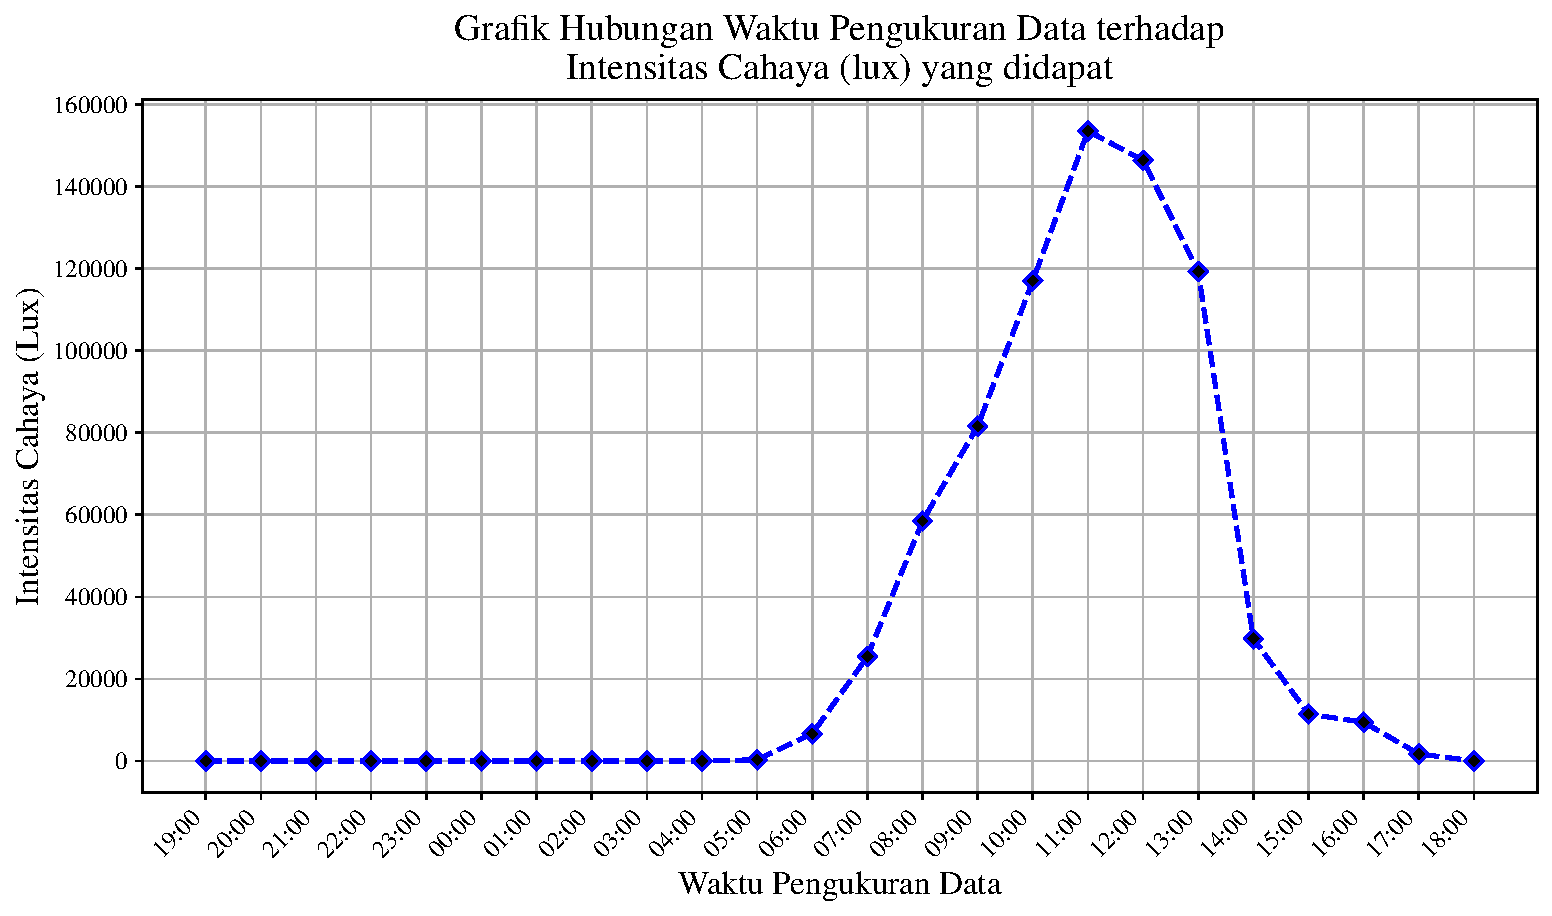
\includegraphics[width=0.95\textwidth]{dataset/grafik waktu vs intensitas.pdf}
    \caption{Grafik waktu pengukuran terhadap hasil ukur intensitas cahaya matahari dengan aplikasi \textit{Pengukur Cahaya}}
    \labfig{waktu-vs-intensitas}
\end{figure}
Berdasarkan \reffig{waktu-vs-intensitas}, intensitas cahaya matahari bervariasi. Pada fase malam hari ke dini hari mulai pukul 18.00 s.d. 04.00 intensitas cahaya matahari adalah 0. Sedangkan mulai pukul 05.00 cahaya matahari mulai terukur dan terus meningkat sampai pada puncaknya dengan rata-rata sebesar 153.540 Lux (pukul 11.00), kemudian mulai menurun kembali sampai nilai terendah pada pukul 17.00. Berdasarkan \reffig{waktu-vs-intensitas} dapat diketahui bahwa waktu tengah hari adalah sekitar pukul 11.00 atau antara 11.00 dan 12.00.

\subsection{Intensitas Cahaya Matahari Terhadap Suhu Udara}
\begin{figure}
    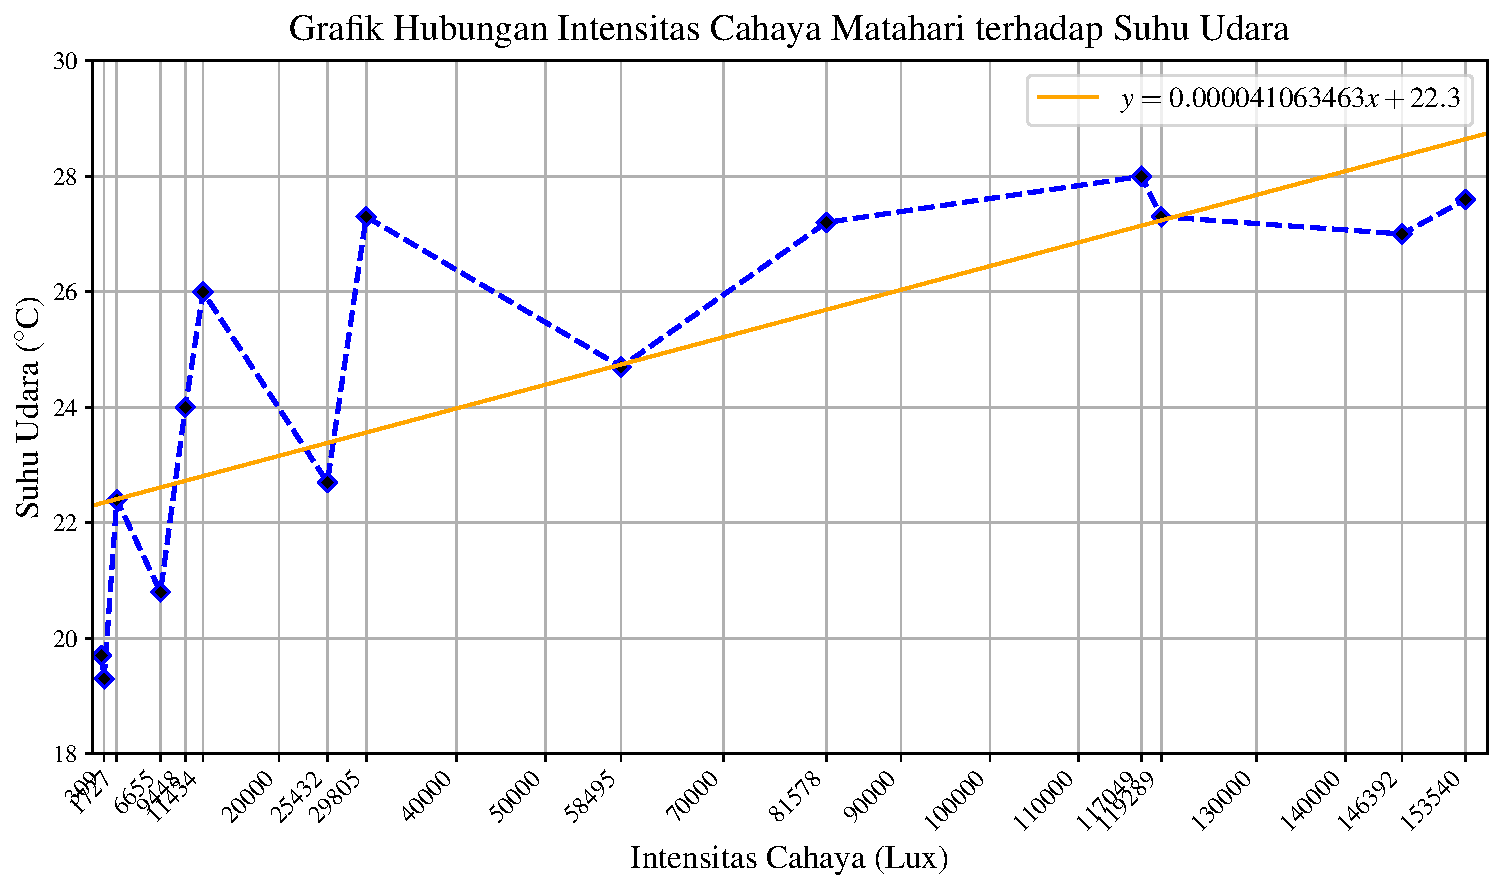
\includegraphics[width=0.95\textwidth]{dataset/grafik intensitas vs suhu.pdf}
    \caption{Grafik intensitas cahaya matahari terhadap suhu udara}
    \labfig{intensitas-vs-suhu}
\end{figure}
Berdasarkan \reffig{intensitas-vs-suhu} diperoleh suhu udara minimum yakni $19,3^\circ$ pada intensitas cahaya matahari 309,3 Lux. Data suhu minimum ini terukur pada pukul 05.00 WIB, Sabtu, 11 November 2023. Sedangkan suhu udara maksimum yakni $28,0^\circ$ pada intensitas cahaya matahari 117.049,3 Lux. Data suhu maksimum ini terukur pada pukul 10.00, Sabtu, 11 November 2023. Dari grafik intensitas cahaya matahari terhadap suhu udara terlihat tren suhu yang meningkat seiring pertambahan intensitas cahaya.

\subsection{Intensitas Cahaya Matahari Terhadap Kelembapan Udara}
\begin{figure}[H]
    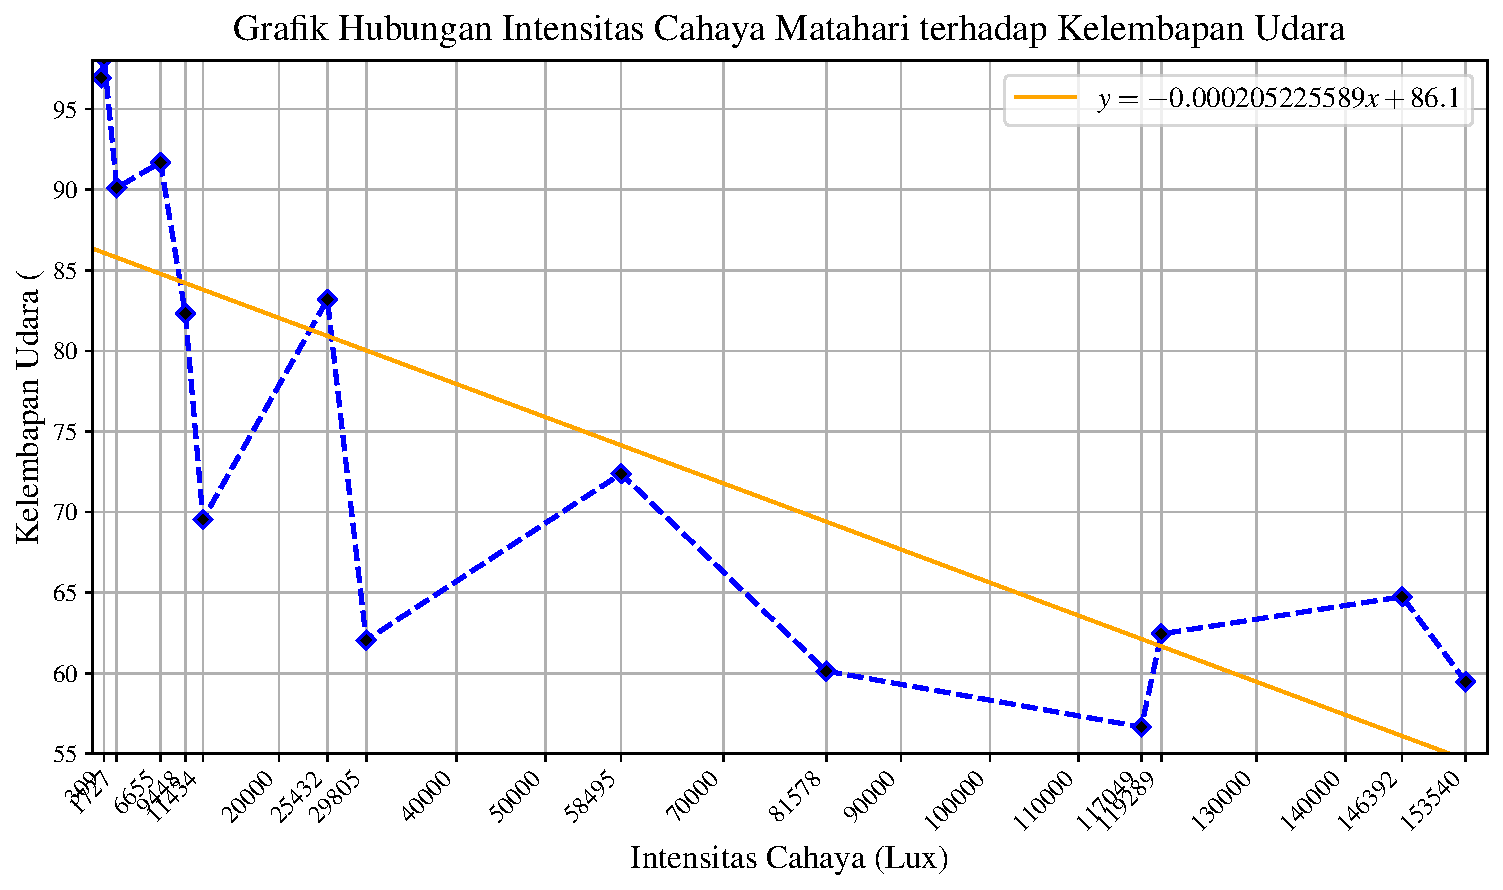
\includegraphics[width=0.95\textwidth]{dataset/grafik intensitas vs kelembapan.pdf}
    \caption{Grafik Intensitas Cahaya Matahari Terhadap Kelembapan Udara}
    \labfig{intensitas-vs-kelembapan}
\end{figure}
Berdasarkan \reffig{intensitas-vs-kelembapan}, diperoleh nilai minimum 56,66\% pada intensitas cahaya matahari 117.049,3 Lux. Data kelembapan minmum ini terukur pada pukul 10.00, Sabtu, 11 November 2023. Sedangkan kelembapan udara maksimum sebesar 98,15\% pada pukul 05.00 WIB dengan intensitas cahaya matahari 309,3 Lux, Sabtu, 11 November 2023. Dari grafik intensitas cahaya matahari terhadap kelembapan udara terlihat tren kelembapan yang menurun seiring pertambahan intensitas cahaya.

